\documentclass[final,hyperref={pdfpagelabels=false}]{beamer}
\usepackage{grffile}
\mode<presentation>{\usetheme{_bauer}}
\usepackage[english]{babel}
\usepackage[latin1]{inputenc}
\usepackage{amsmath, amsthm, amssymb, latexsym}
\usepackage{pifont} % for \ding symbols

%\usepackage{times}\usefonttheme{professionalfonts}  % obsolete
%\usefonttheme[onlymath]{serif}
%\boldmath % macht ALLE Gleichungen automatisch fett
\usepackage[orientation=portrait,size=a0,scale=1.4,debug]{beamerposter}
% change list indention level
% \setdefaultleftmargin{3em}{}{}{}{}{}



% Eigene Befehle und Einstellungen -------------------------
\newcommand{\grayHeader}[1]{\textcolor{koaladarkgray}{{\large #1} \vspace{2ex}}}
\newcommand{\bfBlue}[1]{\textcolor{koaladarkestblue}{\textbf{#1}}}
\newcommand{\blue}[1]{\textcolor{koaladarkestblue}{#1}}
\newcommand{\colHeader}[1]{
  \vspace{-3ex}
  \begin{center}
  \bfBlue{#1}
  \end{center}
  \vspace{-2ex}
  \textcolor{koalablue}{\hrule{\linewidth}}
  \vspace{2ex}
}
% Numbers with circles around it for headers
\usepackage{tikz}
\newcommand*\circled[1]{\tikz[baseline=(char.base)]{
\node[shape=circle,draw,inner sep=2pt] (char) {#1};}}
% Make figures get numbers (Figure 1, ...)
\setbeamertemplate{caption}[numbered]
% Change style of figure caption label
\usepackage[font={footnotesize,it,color=black}]{caption}
\captionsetup[figure]{labelfont={color=black}}
\captionsetup[figure]{labelfont=bf}
% Highlight text parts with a color block with rounded corners
\usepackage{tcolorbox}
\newtcbox{\mybox}{nobeforeafter,colframe=chocolate4,colback=verylightgray,boxrule=2pt,arc=4pt,
  boxsep=0pt,left=6pt,right=6pt,top=6pt,bottom=6pt,tcbox raise base}
% Eigene Befehle Ende --------------------------------------



%\usepackage{snapshot} % will write a .dep file with all dependencies, allows for easy bundling

\usepackage{array,booktabs,tabularx}
\newcolumntype{Z}{>{\centering\arraybackslash}X} % centered tabularx columns
\newcommand{\pphantom}{\textcolor{ta3aluminium}} % phantom introduces a vertical space in p formatted table columns??!!
  
  \listfiles

%%%%%%%%%%%%%%%%%%%%%%%%%%%%%%%%%%%%%%%%%%%%%%%%%%%%%%%%%%%%%%%%%%%%%%%%%%%%%%%%%%%%%%
\graphicspath{{figures/}}

\title{\huge{KOALA: Estimating coalition probabilities}\\[0.5ex]\LARGE{in multi-party electoral systems}}
\author{Alexander Bauer$^{1}$, Andreas Bender$^{1}$, Andr\'e Klima$^{1}$, Helmut K\"{u}chenhoff$^{1}$}
\institute[LMU Munich]{\textit{$^{1}$ Statistical Consulting Unit StaBLab, Department of Statistics, LMU Munich,
Germany} \\[2ex] \texttt{Alexander.Bauer@stat.uni-muenchen.de}}
\date[July 18th, 2018]{July 18th, 2018}

%%%%%%%%%%%%%%%%%%%%%%%%%%%%%%%%%%%%%%%%%%%%%%%%%%%%%%%%%%%%%%%%%%%%%%%%%%%%%%%%%%%%%%
  \newlength{\columnheight}
\setlength{\columnheight}{105cm}


%%%%%%%%%%%%%%%%%%%%%%%%%%%%%%%%%%%%%%%%%%%%%%%%%%%%%%%%%%%%%%%%%%%%%%%%%%%%%%%%%%%%%%

% Begin page ----------------------------------------------
\begin{document}
\begin{frame}
\begin{columns}
\begin{column}{1\textwidth} % 1 Seite, die die ganze Seite einnimmt


% Motivation ---------------------------------------------
\begin{beamercolorbox}[center,wd=\textwidth]{postercolumn}
\begin{minipage}[T]{.95\textwidth}  % tweaks the width, makes a new \textwidth
\begin{block}{\footnotesize Data and Research Question}
  \begin{center}
  \grayHeader{Election poll-based reporting}
  \end{center}

  % Upper columns with general description -----
  \begin{columns}[t]

  \begin{column}{.275\textwidth}
  \colHeader{What's the status quo?}
  Election poll reporting is mostly based on observed mean voter shares.
  \end{column}

  \hspace{-1.5ex}
  \textcolor{LMUlightgray}{\vrule{}}
  \hspace{1.5ex}

  \begin{column}{.275\textwidth}
  \colHeader{So what's wrong?}
  The current style has several shortcomings:
  \begin{enumerate}
    \item Sample uncertainty is insufficiently addressed
    \item The main interest is beyond the simple percentages
  \end{enumerate}
  \end{column}

  \hspace{-1.5ex}
  \textcolor{LMUlightgray}{\vrule{}}
  \hspace{1.5ex}

  \begin{column}{.35\textwidth}
  \colHeader{What do we propose?}
   Bla blub
  \begin{enumerate}
    \item ...
    \item ...
  \end{enumerate}
  \begin{center}
  We want to \bfBlue{shift the focus} from \\[2ex]
  \begin{tabular}{ccc}
  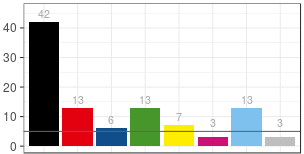
\includegraphics[height=10ex]{figures/motivation_bars}
  &
  to
  &
  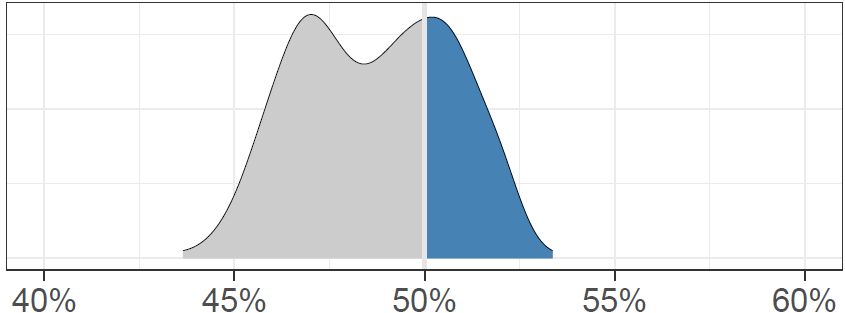
\includegraphics[height=10ex]{figures/motivation_density}
  \\
  incomprehensive & & uncertainty-based \\
  \bfBlue{reporting of observed shares} & & \bfBlue{reporting of probabilities} \\
  \end{tabular}
  \end{center}
  \vspace{1ex}
  \end{column}

  \end{columns}

  \vspace{2ex}
  \textcolor{LMUlightgray}{\hrule{\linewidth}}
  \vspace{2ex}

  % Lower columns with specific examples -----
  \begin{columns}[t]

  \begin{column}{.275\textwidth}
  Based on the last opinion poll before the German federal election 2013
  \\[1ex]
  \begin{center}
  \begin{tabular}{ccccccc}
  \toprule
  \bfBlue{Union} & SPD & Greens & \bfBlue{FDP} & The Left & AfD & Others \\ \midrule
  \bfBlue{40\%} & 26\% & 10\% & \bfBlue{5\%} & 9\% & 4\% & 6\% \\
  \bottomrule
  \end{tabular}
  \end{center}
  \vspace{1ex}
  the parties CDU/CSU (or ''Union``) and FDP -- which planned to jointly form the government -- obtained 50\% (after redistributing party votes $<$5\%).
  \\[2ex]
  Media headline: ZITAT
  \end{column}

  \begin{column}{.025\textwidth}
  \hspace{10ex}
  \huge{\blue{\ding{223}}}
  \end{column}

  \begin{column}{.275\textwidth}
  Example
  \end{column}

  \begin{column}{.025\textwidth}
  \hspace{10ex}
  \huge{\blue{\ding{223}}}
  \end{column}

  \begin{column}{.35\textwidth}
  Example
  \end{column}

  \end{columns}

  \vskip-1ex
\end{block}
\end{minipage}
\end{beamercolorbox}


% Begin main part -----------------------------------
\vspace{2ex}
\begin{columns}[T]

% empty space on left
\begin{column}{.016\textwidth}
\end{column}

\begin{column}{.484\textwidth}
\begin{beamercolorbox}[center,wd=\textwidth]{postercolumn}
\begin{minipage}[T]{.95\textwidth}  % tweaks the width, makes a new \textwidth
% \parbox[t][\columnheight]{\textwidth}{ % must be some better way to set the the height, width and textwidth simultaneously
% Since all columns are the same length, it is all nice and tidy.  You have to get the height empirically

% Main block 1 ---------------------------------------
\begin{block}{\footnotesize \circled{1} Main block 1}
text
\end{block}


% Main block 2 -------------------------------------
\begin{block}{\footnotesize \circled{2} Main block 2}
text
\end{block}



% Begin second column of main part -----------------
\end{minipage}
\end{beamercolorbox}
\end{column}

\begin{column}{.484\textwidth}
\begin{beamercolorbox}[center,wd=\textwidth]{postercolumn}
\begin{minipage}[T]{.95\textwidth}  % tweaks the width, makes a new \textwidth


% Implementation -----------------------------------
\begin{block}{\footnotesize \circled{3} Technical implementation}
\begin{center}

\includegraphics[height=5ex]{figures/Koala_Logo_ohneSchrift}
\\[2ex]
We present results for selected elections on
\bfBlue{\texttt{\href{test}{koala.stat.uni-muenchen.de}}}
\end{center}
\\[2ex]
The implementation is based on several points:
\begin{itemize}
  \item Our approach is implemented in the \bfBlue{R package \texttt{coalitions}}   \item The website is shiny-based
  \item The website update approach is automated
  \item Automatic tweets are sent in the case of new results
  \item For sharing our results we automatically export them to Google Sheets
\end{itemize}

% Footer with software icons
\vspace{1ex}
\textcolor{LMUlightgray}{\hrule{\linewidth}}
\vspace{1ex}
\begin{columns}[t]
  \begin{column}{.15\textwidth}
  \begin{center}
  
\includegraphics[height=5ex]{figures/implementation_r}
  \end{center}
  \end{column}

  \hspace{-1.5ex}
  \textcolor{LMUlightgray}{\vrule{}}
  \hspace{1.5ex}

  \begin{column}{.15\textwidth}
  \begin{center}
  \vspace{1ex}
  
\includegraphics[height=3ex]{figures/implementation_shiny}
  \end{center}
  \end{column}

  \hspace{-1.5ex}
  \textcolor{LMUlightgray}{\vrule{}}
  \hspace{1.5ex}

  \begin{column}{.15\textwidth}
  \begin{center}
  
\includegraphics[height=5ex]{figures/implementation_coalitions}
  \end{center}
  \end{column}

  \hspace{-1.5ex}
  \textcolor{LMUlightgray}{\vrule{}}
  \hspace{1.5ex}

  \begin{column}{.15\textwidth}
  \begin{center}
  
\includegraphics[height=5ex]{figures/implementation_sheets}
  \end{center}
  \end{column}

  \hspace{-1.5ex}
  \textcolor{LMUlightgray}{\vrule{}}
  \hspace{1.5ex}

  \begin{column}{.15\textwidth}
  \begin{center}
  
\includegraphics[height=5ex]{figures/implementation_twitter}
  \end{center}
  \end{column}
\end{columns}
\end{block}

% Communication -----------------------------------
\begin{block}{\footnotesize \circled{4} Communicating our results}
text
\end{block}


% End main part ------------------------------------
\end{minipage}
\end{beamercolorbox}
\end{column}

% empty space on right
\begin{column}{.016\textwidth}
\end{column}

\end{columns}


% Literature ---------------------------------------
\vspace{2ex}
\begin{beamercolorbox}[center,wd=\textwidth]{postercolumn}
\begin{minipage}[T]{.95\textwidth}  % tweaks the width, makes a new \textwidth
\begin{block}{\footnotesize References}
{\footnotesize % begin footnotesize
Bauer, A. (2016). \textit{Auswirkungen der Erdbebenquelldynamik auf den zeitlich\-en Verlauf der Bodenbewegung}. MA thesis. Ludwig-Maximilians-Uni\-versi\-t\"{a}t, Munich, Germany. Available: https://epub.ub.uni-muenchen .de/31976/ \\
% Breuer, A. et al. (2014). Sustained petascale performance of seismic simulations with seissol on supermuc. \textit{Supercomputing - 29th International Conference, ISC 2014}, Leipzig, Germany, 1\,--\,18. Springer International Publishing. \\
Scheipl, F., Gertheiss, J., Greven, S. (2016). Generalized functional additive mixed models. \textit{Electronic Journal of Statistics}, \textbf{10.1}, 1455\,--\,1492. \\
Weiss, A. (2001). Topographic position and landforms analysis. \textit{Poster presentation, ESRI user conference}, San Diego, CA, \textbf{200}. \\
Wood, S.N. et al. (2016). Generalized additive models for gigadata: modelling the UK black smoke network daily data. \textit{Journal of the American Statistical Association}. DOI: 10.1080/01621459.2016.1195744.
} % end footnotesize
\end{block}
\end{minipage}
\end{beamercolorbox}

% End page -----------------------------------------
\end{column} % 1 Spalte, die die ganze Seite einnimmt
\end{columns}
\end{frame}
\end{document}
  
  
  %%%%%%%%%%%%%%%%%%%%%%%%%%%%%%%%%%%%%%%%%%%%%%%%%%%%%%%%%%%%%%%%%%%%%%%%%%%%%%%%%%%%%%%%%%%%%%%%%%%%
    %%% Local Variables: 
    %%% mode: latex
  %%% TeX-PDF-mode: t
  %%% End:
    